\chapter*{End-to-end testing with \CUKE{}}

\ifnotes

    Learning outcomes:
    
    \begin{itemize}
        \item Describe the testing pyramid metaphor
        \item Explain that some manual testing is always desirable, especially exploratory
    \end{itemize}

\fi 

\ifcontent 
    \section*{Testing Pyramid}
    
    The testing pyramid tells us that we're better off with fewer end-to-end tests and more unit tests. This is because end-to-end tests are typically:
    
    \begin{itemize}
        \item slow
        \item brittle
        \item difficult to diagnose when they fail
    \end{itemize}
    
    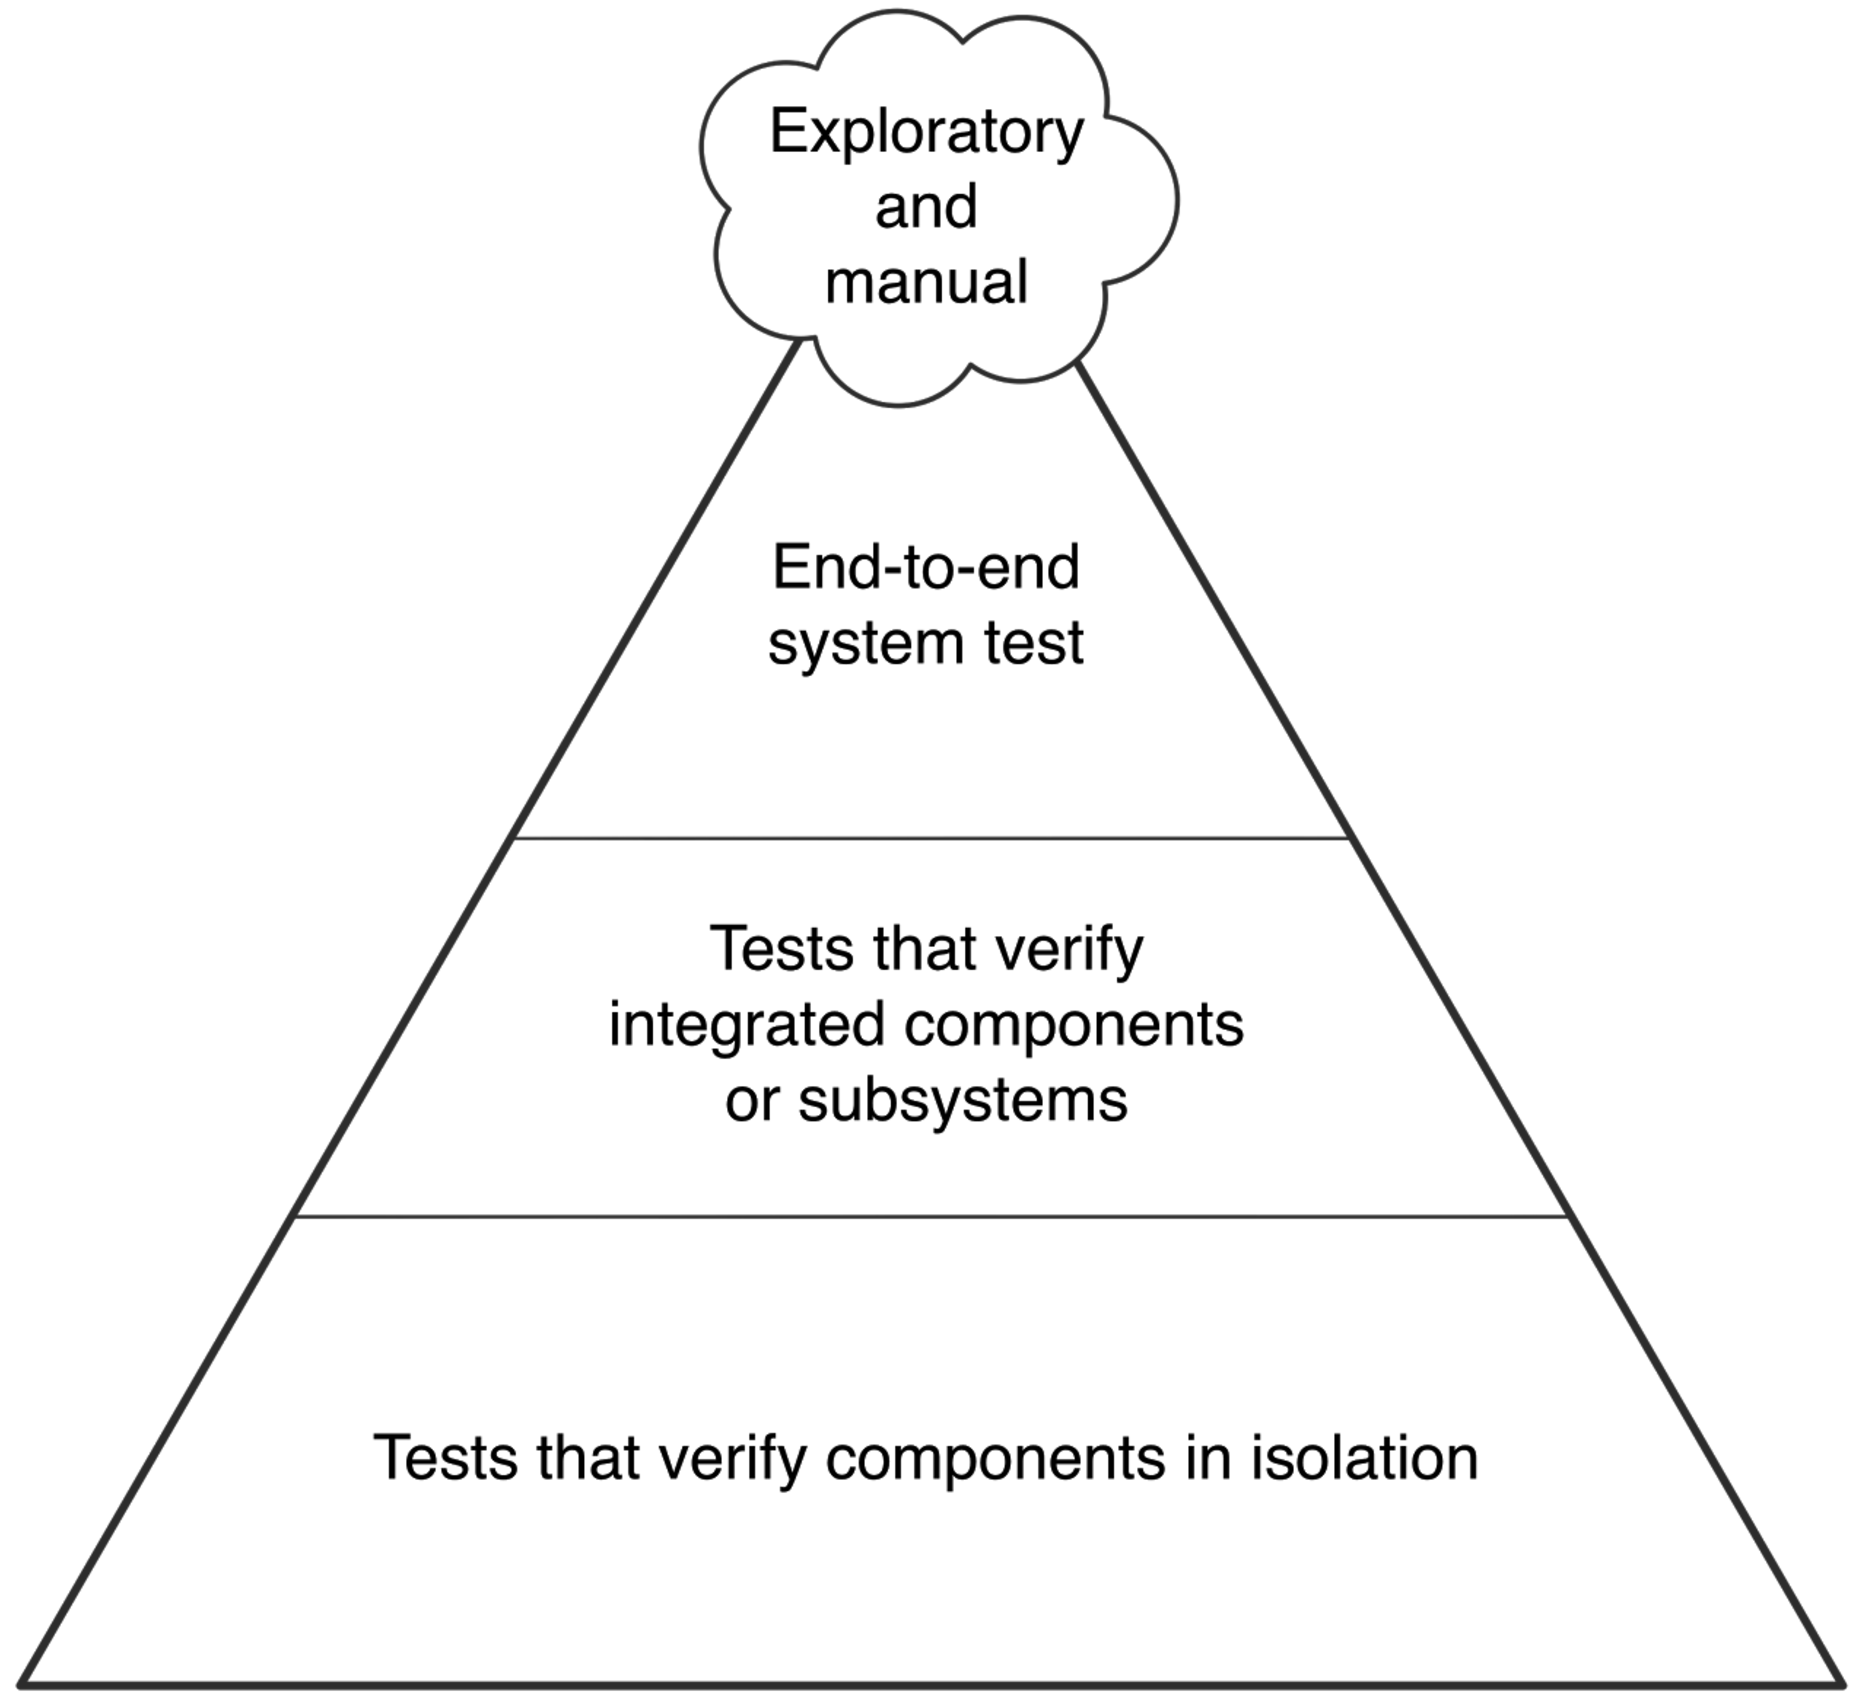
\includegraphics[width=\textwidth]{images/pyramid}
    
    The pyramid also emphasises that there will always be a certain amount of manual and exploratory testing needed.
\fi